% !TEX root = mth727_lecture_notes.tex


\chapter[Some Computations]{Some Computations}
\chaptermark{Some Computations}
\label{SOME COMPUTATIONS CHAPTER}
\thispagestyle{firststyle}

\begin{proposition}
If $X$ is a contractible space then $\pi_{n}(X) = 0$ for all 
$n\geq 0$.  
\end{proposition}

\begin{proof}
Since $X\simeq \ast$ thus $\pi_{n}(X) \cong \pi_{n}(\ast) = 0$.
\end{proof}

\begin{proposition}
\label{PIN FOR CW SKELETON PROP}
If $X$ is a relative CW-complex, $X^{(n)}$ is the $n$-skeleton of $X$, and $x_{0}\in X^{(n)}$, 
then the homomorphism $i_{\ast}\colon \pi_{k}(X^{(n)}, x_{0}) \to \pi_{k}(X, x_{0})$
induced by the inclusion map $i\colon X^{(n)}\hra X$ is  an isomorphism for $k< n$
and an epimorphism for $k=n$.
\end{proposition}

\begin{proof}
We can assume that $x_{0}\in X^{(0)}$. Consider $S^{k}$ as a CW complex with 
a 0-cell $s_{0}\in S^{k}$. By the Cellular Approximation Theorem \ref{CELLAPPROX THM}
any map $\omega\colon (S^{k}, s_{0}) \to (X, x_{0})$ is homotopic (relative to the basepoint)
to cellular map $\omega’\colon (S^{k}, s_{0}) \to (X, x_{0})$. If $k \leq n$ then 
$\omega’(S^{k})\subseteq X^{(n)}$, so $\omega’$ represents an element of 
$\pi_{k}(X^{(n)}, x_{0})$ such that $i_{\ast}([\omega’]) = [\omega]$. This shows that 
$i_{\ast}$ is an epimorphism for $k\leq n$. 

Next, take $[\omega_{0}], [\omega_{1}] \in \pi_{k}(X^{(n)}, x_{0})$. We can assume that 
the maps $\omega_{0}, \omega_{1} \colon (S^{k}, s_{0}) \to (X^{(n)}, x_{0})$ are cellular.
If $i_{\ast}([\omega_{0}]) = i_{\ast}([\omega_{1}])$ then there is a homotopy 
$h\colon S^{k}\times [0, 1] \to X$. Using the Cellular Approximation Theorem 
\ref{CELLAPPROX THM} again, we can assume that this homotopy is a cellular map. 
Since $\dim S^{k}\times [0, 1] = k+1$, we obtain that if $k < n$ then
$h(S^{k}\times [0, 1]) \to X^{(n)}$. Thus $h$ gives a homotopy between $\omega_{0}$
and $\omega_{1}$ in $X^{(n)}$. 
Therefore $[\omega_{0}] = [\omega_{1}] \in \pi_{k}(X^{(n)}, x_{0})$. 
This shows that $i_{\ast}$ is a monomorphism for $k < n$. 
\end{proof}

\begin{corollary}
\label{SN N-1 CONN COROLLARY}
If $k < n$ then $\pi_{k}(S^{n}) = 0$
\end{corollary}

\begin{proof}
A sphere $S^{n}$ can be given a CW-complex structure with one 0-cell and 
one $n$-cell. Then by Proposition \ref{PIN FOR CW SKELETON PROP} for $k< n$ we 
have an epimorphism
\[
\pi_{k}((S^{n})^{(k)}) \to \pi_{k}(S^{n})
\] 
Since $(S^{n})^{(k)} = \ast$, thus $\pi_{k}((S^{n})^{(k)}) = 0$ and so $\pi_{k}(S^{n})=0$.
\end{proof}

\begin{definition}
\label{N CONNECTED SPACE}
A space $X$ is \emph{$n$-connected} if $\pi_{k}(X) = 0$ for all $k\leq n$.
\end{definition}

Corollary \ref{SN N-1 CONN COROLLARY} can be restated by saying that 
the sphere $S^{n}$ is $(n-1)$-connected.

\begin{proposition}
For any space $X$ and $n\geq 0$ the following conditions are equivalent:
\benu
\item[1)] $X$ is $n$-connected.
\item[2)] For any $k\leq n$ and any map $\varphi\colon S^{k}\to X$ there exists 
a map $\xov{\varphi}\colon D^{k+1} \to X$ such that $\xov{\varphi}|_{S^{k}} = \varphi$.
\eenu 
\end{proposition}

\begin{proof}
Follows from Proposition \ref{PIN TRIVAL ELT}.
\end{proof}



By Proposition \ref{PIN FOR CW SKELETON PROP} if $X$ is a CW complex that has only 
one $0$-cell and no $k$-cells for $k\leq n$ (i.e. $X^{(n)} = \ast$) then $X$ is 
$n$-connected. One can show that the opposite is also true, up to a homotopy 
equivalence:  

\begin{proposition}
\label{N SKELETON FOR N CONNECTED PROP}
If $X$ is an $n$-connected CW complex, then there exists a CW complex $Y$ such that 
such that $X\simeq Y$ and $Y^{(n)} = \ast$. 
\end{proposition}

\begin{proof}
We will show inductively that for any $k=0, \dots, n$ there exists a CW complex 
$Y_{k}$ such that $X\simeq Y_{k}$ and $Y_{k}^{(k)} = \ast$. 

Choose a $0$-cell $e^{0}_{0}\in X$.  Since $\pi_{0}(X) = 0$, the space $X$
is path connected. Thus for any $0$-cell $e^{0}_{i}$ we can select a path 
$\omega_{i}\colon [0, 1]\to X$ such that $\omega(0) = e_{0}$ and $\omega(1) = e^{0}_{i}$. 
By the Cellular Approximation Theorem \ref{CELLAPPROX THM}, we can assume that 
$\omega_{i}$ is a path in $X^{(1)}$. We construct a new CW complex 
$Y^{\prime \prime}_{0}$ by attaching cells to $X$ as follows. 

\benu
\item[1)] First, for each $0$-cell $e^{0}_{i}$ we attach to $X$ a $1$-cell 
$e^{1}_{i}$ using the attaching map $\varphi_{i}\colon S^{0} = \{-1, 1\}\to X$
such that $\varphi_{i}(-1) = e^{0}_{0}$ and $\varphi_{i}(1) = e^{0}_{i}$. Let
$Y^{\prime}_{0} = X \cup \bigcup_{i} e^{1}_{i}$ be the CW complex obtained 
in this way.   

\item[2)] In $Y^{\prime}_{0}$ each $0$-cell $e^{0}_{i}$ is 
connected to $e^{0}_{0}$ by two different paths: $\omega_{i}$, and a path  
$\tau_{i}$ that traverses the new cell $e^{1}_{i}$. For each $i$ we attach 
a $2$-cell $e^{2}_{i}$ using an attaching map 
$\psi_{i}\colon S^{1} \to Y^{\prime}_{0}$ that send the lower half circle 
to $\omega_{i}$ and the upper half circle to $\tau_{i}$. Let 
$Y^{\prime \prime}_{0} = Y^{\prime}_{0} \cup \bigcup_{i} e^{2}_{i}$. 
\eenu
\vskip -10mm
\begin{equation*}
\begin{tikzpicture}[scale=1]
\coordinate (A) at (-1.8, -0.3);
\coordinate (B) at (-0.7, 1.1);
\coordinate (C) at (3.2, 1.1);
\coordinate (D) at (3.8, -0.4);
\coordinate (E) at (1, -0.2);
\coordinate (C0) at (1.5, 1);
\coordinate (C1) at (3.3, 0.1);
\coordinate (C2) at (-0.6, 0.0);

\draw[black, fill = mygray1] 
plot [smooth cycle, tension = 0.8] 
coordinates{ (A) (B) (C) (D) };
%\fill (A) circle (0.05) node {A};
%\fill (B) circle (0.05) node {B};
%\fill (C) circle (0.05) node {C};
%\fill (D) circle (0.05) node {D};
\draw[red, very thick, pattern={vertical lines}, pattern color=red] 
(C0) ..controls +(0.3, 3.3)  and +(0, 1).. node[pos=0.4, above] {\small $e^{1}_{i}$} 
(C1) --  cycle;
\draw[red, very thick, pattern={vertical lines}, pattern color=red]
(C0) ..controls +(-0.3, 3.3)  and +(0, 1).. node[pos=0.4, above] {\small $e^{1}_{j}$} 
(C2) -- cycle ;
\draw[very thick] (C0) --  node[below] {\small $\omega_{i}$}  (C1);
\draw[very thick] (C0) --  node[below] {\small $\omega_{j}$}  (C2);
\node[red, fill=white,rounded corners=5pt,inner sep=1pt] at (0.72, 1.6) {\small $e^{2}_{j}$};
\node[red, fill=white,rounded corners=5pt,inner sep=1pt] at (2.2, 1.6) {\small $e^{2}_{i}$};
\node at (-1.9, 1) {\small $X$};
\fill (C0) circle (0.08) node[below] {\small $e^{0}_{0}$};
\fill (C1) circle (0.08) node[right] {\small $e^{0}_{i}$};
\fill (C2) circle (0.08) node[left] {\small $e^{0}_{j}$};
\end{tikzpicture}
\end{equation*}



Notice that $X$ is a deformation retract of $Y^{\prime \prime}_{0}$, so 
the inclusion map $j\colon X \hra Y^{\prime \prime}_{0}$ is a homotopy equivalence. 
Also $A = X^{(0)}\cup \bigcup_{i}e^{1}_{i}$ is a contractible subcomplex of 
$Y^{\prime \prime}_{0}$. By Proposition \ref{CONTR QUOTIENT WITH HEP PROP},
the quotient map $q\colon Y^{\prime \prime}_{0} \to Y^{\prime \prime}_{0}/A$
is a homotopy equivalence. Since $Y^{\prime \prime}_{0}/A$ has a CW complex structure 
with only one $0$-cell we can take $Y_{0} = Y^{\prime \prime}_{0}/A$. 

Next, assume that for some $k\leq n$ we have already constructed 
a CW complex $Y_{k-1}$ such that $X\simeq Y_{k-1}$ and $Y_{k-1}^{(k-1)} = \ast$. 
This means that the $k$-skeleton of $Y_{k-1}$ is given by 
$Y_{k-1}^{(k)} = \bigvee_{i} S^{k}$, with one copy of $S^{k}$ for each
$k$-cell $e^{k}_{i}$ in $Y_{k-1}$. 
Let $\varphi_{j}\colon S^{k} \hra \bigvee_{i} S^{k} \subseteq Y_{k-1}$ be the inclusion 
of the $j$-th copy of $S^{k}$. Since $\pi_{k}(Y_{k-1}) \cong \pi_{k}(X) = 0$, each map 
$\varphi_{i}$ extends to a map $\omega_{i}\colon D^{k+1} \to Y_{k-1}$. We construct a new 
CW complex $Y^{\prime \prime}_{k}$ by attaching cells to $Y_{k-1}$ as follows.

\benu
\item[1)] First, for each $i$ we attach a $(k+1)$-cell  $e^{k+1}_{i}$ using
$\varphi_{i}\colon S^{k} \to Y_{k-1}$ as the attaching map. 
Let $Y^{\prime}_{k} = Y_{k-1} \cup \bigcup_{i} e^{k+1}_{i}$ be the 
CW complex obtained in this way.   

\item[2)] For each $i$ we have now two maps $D^{k+1}\to Y^{\prime}_{k}$:
the map $\omega_{i}$, and the characteristic map $\tau_{i}$ of the cell $e^{k+1}_{i}$.
Using these maps we attach, for each $i$, a $(k+2)$-cell $e^{k+2}_{i}$, 
using an attaching map $\psi_{i}\colon S^{k+1} \to Y^{\prime}_{k}$ that sends the 
lower hemisphere of $S^{k+1}$ to $\omega_{i}$ and the upper hemisphere to $\tau_{i}$. 
Let $Y^{\prime \prime}_{k} = Y^{\prime}_{k} \cup \bigcup_{i} e^{2}_{i}$. 
\eenu

As before, we observe that $Y_{k-1}$ is a deformation retract of $Y^{\prime \prime}_{k}$, 
and that $A = Y_{k-1}^{(k)}\cup \bigcup_{i} e^{k}_{i}$ is a contractible subcomplex
of $Y^{\prime \prime}_{k}$. Therefore we obtain a 
$X\simeq Y_{k-1} \simeq Y^{\prime \prime}_{k}\simeq Y^{\prime \prime}_{k}/A$. It remains
to notice that the space $Y_{k} = Y^{\prime \prime}_{k}/A$ has a CW-complex structure 
such that $Y_{k}^{(k)} = \ast$. 

\end{proof}



\begin{nn}{\bf Homotopy groups and coverings.}
Recall that covering of a space $X$ is a map $p\colon T\to X$ which is locally 
homeomorphic to the projection map $\pr_{1}\colon U\times D \to U$ for some discrete 
space $D$. 
\end{nn}


\begin{equation*}
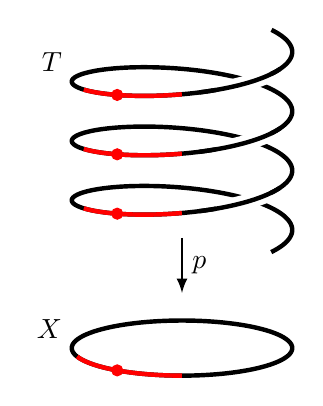
\begin{tikzpicture}[scale=1,
    d1/.style= {postaction={decorate}, decoration={markings, mark=at position 0.2 with {\arrow{stealth}}}},
]

\def\a{1.4}
\def\b{0.35}
\def\c{0.12}

% covering space
\draw[line width=1.6pt,  domain= {-0.2*pi}:{6.2*pi}, samples=500] 
 plot ({\a*cos(deg(\x))}, {\b*sin(deg(\x)) + \c*\x} );

% intersections
\foreach \s in {1, 3, 5}{
\draw[line width = 5.6pt, white, domain= {{(\s + 0.6)*pi}}:{{(\s + 0.8)*pi}}, samples=100]
 plot ({\a*cos(deg(\x))}, {\b*sin(deg(\x)) + \c*\x} );
\draw[line width = 1.6pt, domain= {{(\s + 0.55)*pi}}:{{(\s + 0.85)*pi}}, samples=100]
 plot ({\a*cos(deg(\x))}, {\b*sin(deg(\x)) + \c*\x} );
 }
  
% red pieces
\foreach \s in {1, 3, 5}{
\draw[line width = 1.6pt, red, domain= {{(\s + 0.15)*pi}}:{{(\s + 0.5)*pi}}, samples=100]
 plot ({\a*cos(deg(\x))}, {\b*sin(deg(\x)) + \c*\x} );
}
% red points
\foreach \s in {1, 3, 5}{
\coordinate (X) at ({\a*cos(deg((\s + 0.3)*pi))}, 
{\b*sin(deg((\s + 0.3)*pi)) + \c*((\s + 0.3)*pi)});
\filldraw[red] (X) circle (0.07);
}

\node[anchor=south east] at ({\a*cos(deg(5*pi))}, {\b*sin(deg(5*pi)) + \c*5*pi}) {$T$};

% arrow
\draw[thick, ->, >=latex] (0.0, -0.1) -- node[anchor=west] {$p$} (0.0, -0.8);

% bottom circle
\draw[line width=1.6pt,  domain= {0}:{2*pi}, samples=500] 
 plot ({\a*cos(deg(\x))}, {\b*sin(deg(\x)) - 1.5});
% red piece
\draw[line width = 1.6pt, red, domain= {{(1 + 0.1)*pi}}:{{(1 + 0.5)*pi}}, samples=100]
 plot ({\a*cos(deg(\x))}, {\b*sin(deg(\x)) - 1.5});
% red point
\coordinate (X) at ({\a*cos(deg(1.3*pi))}, {\b*sin(deg(1.3*pi)) - 1.5});
\filldraw[red] (X) circle (0.07);

\node[anchor=south east] at ({\a*cos(deg(pi))}, {\b*sin(deg(pi)) - 1.5}) {$X$};
\end{tikzpicture}
\end{equation*}



Recall also, that one of the main properties of coverings is the following fact: 

\begin{LIFTCRITTHM}
\label{LIFTINGCRIT THM}
Let $p\colon T\to X$ be a covering, let $x_{0}\in X$ and let $\ntilde{x}_{0}\in p^{-1}(x_{0})$. Assume that $Y$
is a connected and locally path connected space and let $y_{0}\in Y$.  A map $f\colon (Y, y_{0}) \to (X, x_{0})$
has a lift $\ntilde{f}\colon (Y, y_{0}) \to (T, \ntilde{x}_{0})$ if and only if 
$f_{\ast}(\pi_{1}(Y, y_{0})) \subseteq p_{\ast}(\pi_{1}(T, \ntilde{x}_{0}))$. 
\begin{equation*}
\begin{tikzpicture}[baseline=(current  bounding  box.center)]
\matrix (m) 
[matrix of math nodes, row sep= 2.5em, column sep=3em, text height=1.5ex, text depth=0.25ex]
{
   &  T \\
Y & X & \\ 
};
\path[->, thick, font=\scriptsize]
(m-2-1) 
edge node[auto] {$\ntilde{f}$} (m-1-2)
edge node[below] {$f$} (m-2-2)
(m-1-2) 
edge node[auto] {$p$} (m-2-2)
;
\end{tikzpicture}
\end{equation*}
Moreover, if a lift $\ntilde{f}$ exists, then it is unique.
\end{LIFTCRITTHM}

Recall that for any covering $p\colon (T, \ntilde{x}_{0}) \to (X, x_{0})$
the induced homomorphism 
$p_{\ast}\colon \pi_{1}(T, \ntilde{x}_{0}) \to \pi_{1}(X, x_{0})$
is a monomorphism. 
Using Theorem \ref{LIFTINGCRIT THM} we can generalize this as follows:

\begin{proposition}
\label{COVERING PIN PROP}
If $p\colon T\to X$ is a covering, $x_{0}\in X$ and $\ntilde{x}_{0}\in p^{-1}(x_{0})$, then 
the induced homomorphism 
\[
p_{\ast}\colon \pi_{n}(T, \ntilde{x}_{0}) \to \pi_{n}(X, x_{0})
\]
is an isomorphism for all $n>1$. 
\end{proposition}

\begin{proof}
Let $n>1$  and $\omega \colon (S^{n}, s_{0}) \to (X, x_{0})$ represents an element of 
$\pi_{n}(X, x_{0})$. Since $\pi_{1}(S^{n}) = 0$, by Theorem \ref{LIFTINGCRIT THM}
there exists a map $\widetilde\omega \colon (S^{n}, s_{0}) \to (T, \ntilde{x}_{0})$
such that $p\widetilde\omega = \omega$. This shows that 
$p_{\ast}\colon \pi_{n}(T, \ntilde{x}_{0}) \to \pi_{n}(X, x_{0})$ is onto. 

Next, assume that $\omega_{0}, \omega_{1}\colon (S^{n}, s_{0}) \to (T, \ntilde{x}_{0})$
are maps such that $p_{\ast}([\omega_{0}]) = p_{\ast}([\omega_{1}])$. 
This means that there exists a basepoint preserving homotopy 
$h\colon S^{n}\times [0, 1] \to X$, such that $h_{0} = p\omega_{0}$, $h_{1} = p\omega_{1}$. 
Since $S^{n}\times [0, 1] \simeq S^{n}$ we have 
$\pi_{1}(S^{n}\times [0, 1])\cong \pi_{1}(S^{n}) = 0$. Thus by 
Theorem \ref{LIFTINGCRIT THM}, there exists a homotopy 
$\widetilde h\colon S^{n}\times [0, 1] \to T$ such that $p\widetilde h = h$ and
$\widetilde h(s_{0}, 0) = \ntilde{x}_{0}$. Using the uniqueness of lifts, one can check 
that $\widetilde h_{0} = \omega_{0}$ and $\widetilde h_{1} = \omega_{1}$, and that 
the homotopy $\widetilde h$ preserves the basepoint (exercise). It follows that 
$[\omega_{0}] = [\omega_{1}]$ in $\pi_{1}(T, \ntilde{x}_{0})$. Therefore $p_{\ast}$
is a monomorphism. 


\end{proof}



\begin{example}
\label{PIN S1 EXAMPLE}
$\pi_{n}(S^{1}) = 0$ for all $n>1$. 

Indeed, universal covering of $S^{1}$ is given by a map $p\colon \R \to S^{1}$. 
Since $\R$ is a contractible space, by Proposition \ref{COVERING PIN PROP}
for $n>1$ we obtain
\[
\pi_{n}(S^{1}) \cong \pi_{n}(\R) = 0
\]
\end{example}


\begin{example}
\label{PIN S1vSm EXAMPLE} If $m > 1$ then 
$\pi_{n}(S^{1}\vee S^{m}) \cong \pi_{n}(\bigvee_{i\in\Z} S^{m})$ for all $n > 1$. 

To see this, notice that the universal covering of $S^{1}\vee S^{m}$ is
the space $\widetilde X$ obtained by attaching copies of $S^{m}$ at all integer points 
of the real line:

\begin{equation*}
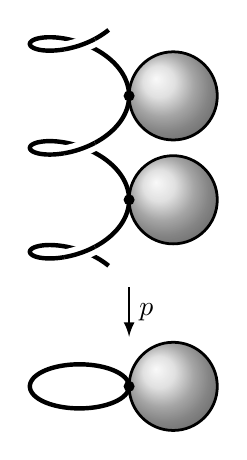
\begin{tikzpicture}[scale=0.7,
    d1/.style= {postaction={decorate}, decoration={markings, mark=at position 0.2 with {\arrow{stealth}}}},
]
\draw[line width=1.6pt,  domain= {0.3*pi}:{5.7*pi}, samples=500] 
 plot ({0.9*cos(deg(\x))}, {0.5*sin(deg(\x)) + 0.3*\x} );

 
 \draw[line width = 5.6pt, white, domain= {1.4*pi}:{1.6*pi}, samples=100]
 plot ({0.9*cos(deg(\x))}, {0.5*sin(deg(\x)) + 0.3*\x} );
\draw[line width = 1.6pt, domain= {1.4*pi}:{1.6*pi}, samples=100]
 plot ({0.9*cos(deg(\x))}, {0.5*sin(deg(\x)) + 0.3*\x} );
 
\draw[line width = 5.6pt, white, domain= {3.4*pi}:{3.6*pi}, samples=100]
 plot ({0.9*cos(deg(\x))}, {0.5*sin(deg(\x)) + 0.3*\x} );
\draw[line width = 1.6pt, domain= {3.4*pi}:{3.6*pi}, samples=100]
 plot ({0.9*cos(deg(\x))}, {0.5*sin(deg(\x)) + 0.3*\x} );
 
 \draw[line width = 5.6pt, white, domain= {5.4*pi}:{5.6*pi}, samples=100]
 plot ({0.9*cos(deg(\x))}, {0.5*sin(deg(\x)) + 0.3*\x} );
\draw[line width = 1.6pt, domain= {5.4*pi}:{5.6*pi}, samples=100]
 plot ({0.9*cos(deg(\x))}, {0.5*sin(deg(\x)) + 0.3*\x} );
 
\coordinate (C1) at ({0.9*cos(deg(2*pi)) + 0.8}, {0.5*sin(deg(2*pi)) + 0.3*2*pi});
\coordinate (T1) at ({0.9*cos(deg(2*pi))}, {0.5*sin(deg(2*pi)) + 0.3*2*pi});
\shade[ball color = gray!40, opacity = 0.8] (C1) circle (0.8);
\draw[line width=1pt] (C1) circle (0.8);
\fill (T1) circle (0.1);

\coordinate (C2) at ({0.9*cos(deg(4*pi)) + 0.8}, {0.5*sin(deg(4*pi)) + 0.3*4*pi});
\coordinate (T2) at ({0.9*cos(deg(4*pi))}, {0.5*sin(deg(4*pi)) + 0.3*4*pi});
\shade[ball color = gray!40, opacity = 0.8] (C2) circle (0.8);
\draw[line width=1pt] (C2) circle (0.8);
\fill (T2) circle (0.1);


\draw[thick, ->, >=latex] (0.9, 0.3) -- node[anchor=west] {$p$} (0.9, -0.6);

\draw[line width=1.6pt,  domain= {0}:{2*pi}, samples=500] 
 plot ({0.9*cos(deg(\x))}, {0.4*sin(deg(\x)) - 1.5});
\coordinate (C0) at ({0.9 + 0.8}, -1.5);
\coordinate (T0) at  ({0.9}, -1.5);
\shade[ball color = gray!40, opacity = 0.8] (C0) circle (0.8);
\draw[line width=1pt] (C0) circle (0.8);
\fill (T0) circle (0.1);

\end{tikzpicture}
\end{equation*}

The space $\widetilde X$ can be given the structure of a CW complex, such that the real line 
$\R$ is its subcomplex. Since $\R\simeq \{\ast\}$, by Theorem \ref{HEP REL CW THM} we
have $\widetilde X \simeq \widetilde X/\R \cong \bigvee_{i\in \Z} S^{m}$. Therefore for $n > 1$
we obtain 
\[
\pi_{n}(S^{1}\vee S^{m}) \cong \pi_{n}(\widetilde X) \cong \pi_{n}(\textstyle\bigvee_{i\in \Z} S^{m})
\]
\end{example}

\begin{note}
\label{SAME HOMOT GPS NO EQUIV NOTE}
Example \ref{PIN S1vSm EXAMPLE} can be used to show that if $X$,  $Y$ are spaces such that
$\pi_{n}(X) \cong \pi_{n}(Y)$ for all $n\geq 0$, then this does not imply 
that $X\simeq Y$. 

Take, for example, $X = S^{1}\vee S^{m}$ for some $m> 1$, and let 
$Y = S^{1}\vee S^{m} \vee S^{m}$. These spaces are not homotopy equivalent, since they 
have different homology groups: 
$H_{m}(X; \Z) \cong \Z$ and $H_{m}(Y; \Z) \cong \Z\oplus \Z$.

On the other hand, since both these spaces are path connected, 
we have $\pi_{0}(X) \cong \pi_{0}(Y)\cong \{\ast\}$. 
Also, since $\pi_{1}(S^{m}) = 0$, thus by 
van Kampen’s theorem we get $\pi_{1}(X) \cong \pi_{1}(S^{1}) \cong \pi_{1}(Y)$.

The universal covering space $\widetilde Y$ of $Y$ is the space obtained by attaching 
$S^{m}\vee S^{m}$ at all integer points of $\R$. Using the same argument as in 
Example \ref{PIN S1vSm EXAMPLE}, we obtain 
$\widetilde Y \simeq \bigvee_{i\in \Z} (S^{m}\vee S^{m}) \cong \bigvee_{i\in \Z} S^{m}$. 
Therefore for $n\geq 2$ we have
\[
\pi_{n}(X) \cong \pi_{n}(\textstyle\bigvee_{i\in \Z} S^{m}) \cong \pi_{n}(Y)
\]

\end{note}





\begin{theorem}
\label{PIN  PROD THM}
For a family ${(X_{i}, \xov{x}_{i})}_{i\in I}$ be a family of pointed spaces there is 
an isomorphism
$$\pi_{n}\left(\prod_{i\in I} X_{i}, \ (\xov{x}_{i})_{i\in I}\right) \cong  \prod_{i\in I} \pi_{n}(X_{i}, \xov{x}_{i})$$
\end{theorem}


\begin{proof}
For $j\in I$ let $p_{j}\colon \prod_{i\in I} X_{i} \to X_{j}$ denote the projection 
onto the $j$-th factor. The induced homomorphisms $p_{j\ast}$ define a homomorphism:
\[
\prod_{i\in I}p_{i\ast} \colon
\pi_{n}\left(\prod_{i\in I} X_{i}, \ (\xov{x}_{i})_{i\in I}\right) \to  
\prod_{i\in I} \pi_{n}(X_{i}, \xov{x}_{i})
\]

To obtain a homomorphism going in the opposite direction, let
$([\omega_{i}])_{i\in I}$ be an element of $\prod_{i\in I} \pi_{n}(X_{i}, \xov{x}_{i})$. 
Then each $\omega_{i}$ is a map $\omega_{i}\colon (S^{n}, s_{0}) \to (X_{i}, \xov{x}_{i})$. 
Take the product map 
\[
\prod_{i\in I}\omega_{i} \colon (S^{n}, s_{0}) \to (\prod_{i} X_{i}, \xov{x}_{i})
\]
One can check that the assignment 
$([\omega_{i}])_{i\in I} \mapsto [\prod_{i\in I}\omega_{i}]$
gives a well-defined homomorphism
\[
g\colon \prod_{i\in I} \pi_{n}(X_{i}, \xov{x}_{i}) \to 
\pi_{n}\left(\prod_{i\in I} X_{i}, \ (\xov{x}_{i})_{i\in I}\right)
\]
and that the compositions $g\circ \prod_{i\in I}p_{i\ast}$ and 
$\prod_{i\in I}p_{i\ast} \circ g$ are identity homomorphisms (exercise).
\end{proof}

\begin{example}
Since $\pi_{1}(S^{1}) \cong \Z$ and $\pi_{n}(S^{1}) = 0$ for $n > 1$, 
thus for any set $I$ we have 
\[
\pi_{n}\left(\prod_{i\in I} S^{1}\right) \cong
\begin{cases}
\prod_{i\in I} \Z & \text{for $n=1$} \\[2mm]
0 & \text{for $n>1$} \\
\end{cases}
\]
\end{example}



